\chapter{The MicroBooNE Experiment}\label{ch:microboone}
The purpose of this chapter is to discuss and understand the details of the MicroBooNE detector. A thorough understanding of MicroBooNE and the technology behind liquid argon time projection chambers is important for understanding results as well as understanding how images were made for use in deep learning efforts that will be outlined in later chapters.   

\section{Liquid argon time projection chambers}
Liquid Argon Time Projection Chambers (LArTPCs) are an exciting detector technology that provide excellent imaging and particle identification, and are now being used to study neutrinos. The Time Projection Chamber (TPC) was first invented by Nygren in 1974 \cite{nygren} and the proposal for a LArTPC for neutrino physics was made by Rubbia \cite{rubbia} and in 1977 the ICARUS collaboration implemented the idea \cite{icarus}. A LArTPC is a three-dimensional imaging detector that uses planes of wires at the edge of an active volume to read out an interaction. When a neutrino interacts with an argon atom, the charged particles that are produced ionize the LAr as they travel away from the interaction. By placing a uniform electric field throughout the LAr volume, the ionization drifts towards a set of anode planes, which consist of wires spaced very closely together collecting the ionized charge. The ionized charge is then read out by electronics connected to the anode wires. The collected ionization creates an image of what happened in the detector on each anode plane. The drift time of the ionization relative to the time of the original signal allows the signal to be projected back along the drift coordinate, hence the name TPC. Having very small distances between each wire within an anode plane allows for very fine granularity and detail to be captured, and having multiple wire planes at different angles provides independent two-dimensional views that can be combined into a three-dimensional picture of the interaction. Once the charge signal is created on the anode planes, software analysis packages identify particles in the detector by using deposited energy on the wires along their track length. 

The 30 year development of the ICARUS detector has led to LArTPCs being used to study cosmic rays \cite{lartpc_cosmic}, solar neutrinos \cite{lartpc_solar} and accelerator neutrinos \cite{lartpc_accelerator} detectors. The ArgoNeuT experiment at Fermilab was the first United States based liquid argon neutrino program that has since produced short-baseline $\nu-Ar$ cross-section measurements in the NUMI beam-line \cite{argoneut1}-\cite{argoneut4}. The MicroBooNE experiment is the second beam experiment in the US based LArTPC neutrino program and will be discussed thoroughly in the next sections.  

The next phases of the liquid argon neutrino program are under way and are the Fermilab Short Baseline Neutrino (SBN) program \cite{sbn} and the Deep Underground Neutrino Experiment (DUNE) \cite{dune}. The SBN program will include three LArTPC detectors, including the MicroBooNE detector, on the Booster Neutrino Beam (BNB) to do multiple-baseline oscillation measurements. The detector closest to the beam will be the \sim 100 ton Short Baseline Neutrino Detector (SBND)\cite{sbnd} at 150 m and the detector furthest is the 600 ton ICARUS T600 \cite{icarus_t600} detector positioned at 600 m. The DUNE collaboration will deliver a neutrino beam 1300 km from Fermilab to the DUNE LArTPC detector at Homestake, SD. DUNE will study the leptonic CP phase, $\delta_{cp}$, as well as measure neutrino and anti-neutrino oscillations. 
\section{The MicroBooNE Time Projection Chamber}
MicroBooNE \cite{microboone}(Micro Booster Neutrino Experiment) is a ~89 ton active volume (180 ton total mass) LArTPC which is then inserted into a cylindrical cryostat. MicroBooNE is on the BNB line axis stationed at Fermilab in Batavia, Illinois. Understanding LArTPC technology and detector physics is necessary to build a LArTPC the size of DUNE, and MicroBooNE has made many advances in developing this technology\cite{noisechar} \cite{michel}. 

MicroBooNE's Time Projection Chamber (TPC) is 10.3 m long (beam-line direction), 2.3 m high and 2.5 m wide (which corresponds to the drift distance). The TPC is shown in figure \ref{fig:tpc}. MicroBooNE is the largest LArTPC currently running in the world. This LArTPC has 3 wire planes: 1 plane that collects the ionization in the wires and is $0^{\circ}$ to the vertical with 3456 wires spaced 3 mm apart, and 2 planes where the ionization drifts past and induces a signal on the wires which are $\pm 60^{\circ}$ to the vertical. Each induction plane has 2400 wires also spaced 3 mm apart. Each plane has a spacing also of 3 mm from each-other. The first two planes are the induction planes and the last is the collection. The 270 V/cm electric field of the TPC is created using 64 stainless steel tubes shaped into rectangles around the TPC and held in place by G10 to form a field cage. The cathode is biased at a high voltage of -70 kV and this voltage is stepped down across the field cage tubes using a voltage divider chain with an equivalent resistance of 240 $\text{M}\ohm$ between the tubes. The field cage tubes are separated by 4 cm from center to center. The electron drift distance is 2.5 m in the $\hat{x}$ direction with a drift time of 2.3 ms. Maintaining high charge yield is done by continuously recirculating and purifying the argon. 
\begin{figure}[htp!]
\centering
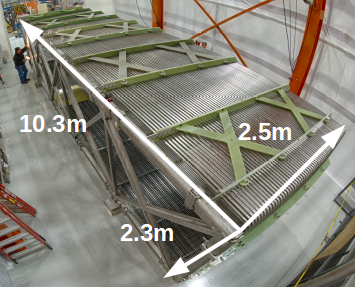
\includegraphics[width=.5\textwidth]{figs/detector1.png}
\caption{MicroBooNE TPC}
\label{fig:tpc}
\end{figure}

MicroBooNE's light collection system is a crucial part for 3D reconstruction of all particle interactions in the LArTPC. The initial interaction time, $t_0$, and initial drift coordinate, $x_0$, are not known from the TPC alone. For beam events, the accelerator clock is used to determine $t_0$ of the interaction and the $x_0$ can be inferred using drift time. Non-beam events, however, do not have this capability, which is why scintillation light from an interaction is used. The $\nu-Ar$ interaction produces scintillation light which is collected by photomultiplier tubes (PMTs) which allows the exact time, $t_0$ of the neutrino interaction to be determined. The scintillation light created propagates within nanoseconds to the light collection system compared to the milliseconds it takes the ionized electrons from the interaction to reach the anode wire planes. Therefore we can precisely know where along the drift direction the particle interaction first took place. The scintillation light is also localized, so combining the PMT information with the wire plane information allows for background rejection of cosmics happening outside the beam timing window.  


The light collection system is made up of 32 Hammamatsu R5912-02mod cryogenic PMTs with a diameter of 8-inches. The PMTs are located behind the 3 wire anode planes and provides 0.85\% photo-cathode coverage. Each PMT has an acrylic plate mounted in front of it that is coated with a wave-length shifting material called tetraphenyl-butadiene (TPB). The acrylic plates take in the scintillation light, at 128 nm, and re-emits it at wavelengths visible to the PMTs, with a peak at 425 nm. 

Both the light collection system and the TPC create analog signals that is read out and digitized by the electronics system. The process requires amplification and shaping of the signal which then goes to the data acquisition (DAQ) software for writing of the digitized data to disk. The anode plane wires are connected to detector specific circuit boards (ASICS) that are submerged and operate inside the liquid argon volume. These ASICS send amplified signal to 11 feed-throughs where further amplification of the signal happens outside the cryostat. The signal is received by custom LArTPC readout modules distributed over nine readout crates which do the digitization. The TPC wires are digitized at 16 MHz then downsampled to 2 MHz. The TPC system reads out 4 frames of wire signal data per event, 1 frame before a trigger, 1 frame during the trigger, and 2 frames after the triggered frame. The four frames allows for identification of a neutrino interaction as well as cosmic background rejection. The process of digitization is similar for the light collection system. Each PMT signal undergoes a shaping with a 60 ns  peaking time for digitization of multiple samples. The digitization occurs at 64 MHz but are not read out continuously during the TPC readout time. Only shaped PMT signal samples above a small threshold are read out and saved. Both the TPC and PMT readouts are initiated via triggers on a separate trigger board located in a warm electronics crate. The timing trigger is created by a timing signal from the BNB accelerator which is shaped and sent to the trigger board. The PMT trigger is generated when the PMT signal multiplicity is greater than 1 and the summed PMT pulse-height is more than 2 photo-electrons summed up over all PMT channels. When the trigger board gets both a timing trigger and a PMT trigger in coincidence, at BNB trigger is then generated by the board. This signal is then passed to all readout crates initiating the readout of data. The data is then sent to the DAQ software which then saves the data to disk into one event memory.

\section{MicroBooNE's Physics Goals} 
\subsection{The low-energy excess}
The primary goal of the MicroBooNE experiment is to study and investigate the low-energy excess seen in MiniBooNE and shown in figure \ref{fig:lee} \cite{miniboone1} \cite{miniboone2}. MiniBooNE was on the BNB which produced both $\nu_{mu}$ and $\overline{\nu_{\mu}}$ modes. MiniBooNE searched for appearances of $\nu_e$ in neutrino mode and $\overline{\nu_e}$ in anti-neutrino mode. In both modes, MiniBooNE observed an excess over the expected backgrounds at low energies. MiniBooNE's low-energy excess is either mis'ided photons from background or electrons from a $\nu_e$ appearance. MicroBooNE has the capability of confirming or denying this excess as electrons or photons due to the detector being in the same beam, having a similar baseline, and lastly the detector being able to clearly distinguish between electrons and photons. LArTPCs use the topology of events as well as energy loss near the vertex to differentiate between single $e^-$ tracks and photon-induced induced pair production $\gamma \rightarrow e^+e^-$, which wasn't possible in MiniBooNE, a cherenkov detector. This technique has been shown in the ArgoNeuT detector and a side by side comparison of both event types in a LArTPC can be seen in figure \ref{fig:egamma}. An excess in electrons would point towards new oscillation physics beyond the standard model, while photons would be within the standard model. MicroBooNE will observe a 4-5$\sigma$ signal.  

\begin{figure}[htp!]
\centering
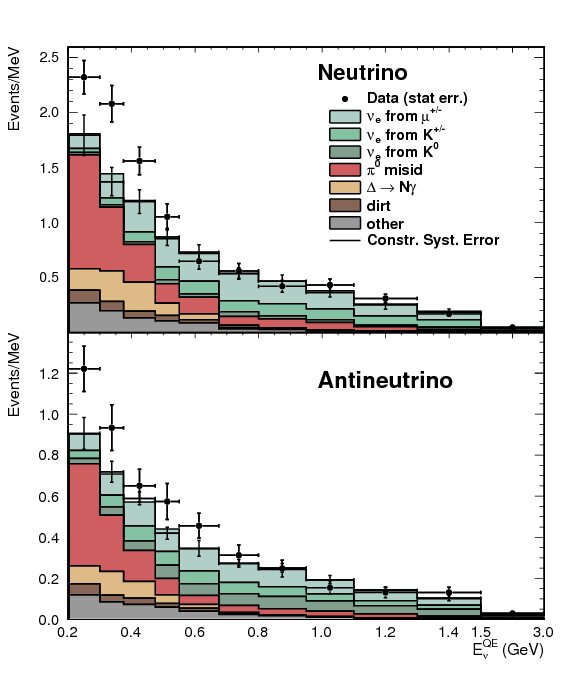
\includegraphics[width=.5\textwidth]{figs/lee.png}
\caption{Low Energy excess seen in MiniBooNE \cite{miniboone1}}
\label{fig:lee}
\end{figure}

\begin{figure}[htp!]
\centering
	\begin{subfigure}[t]{.475\textwidth}
	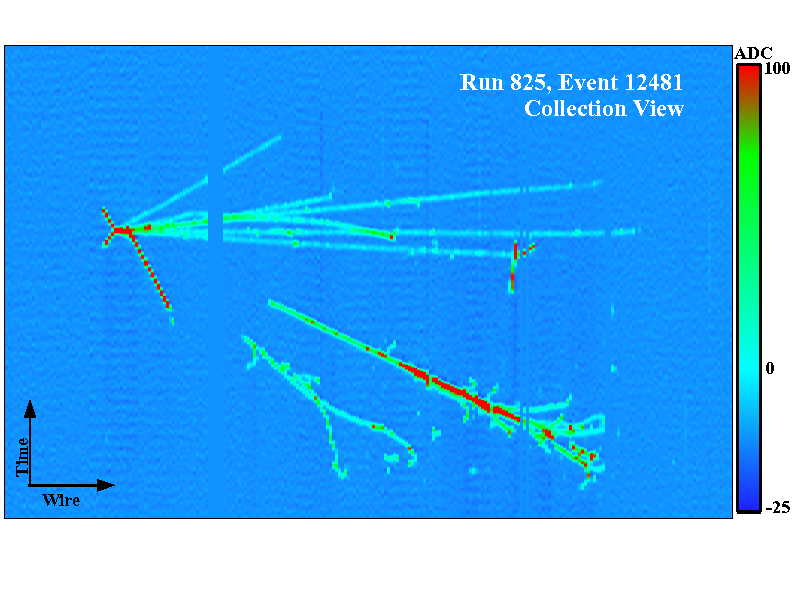
\includegraphics[width=\textwidth]{figs/gamma.png}
	\caption{Example of an event with two gamma candidates.}
	\label{fig:gamma}
	\end{subfigure}
	\begin{subfigure}[t]{.475\textwidth}
	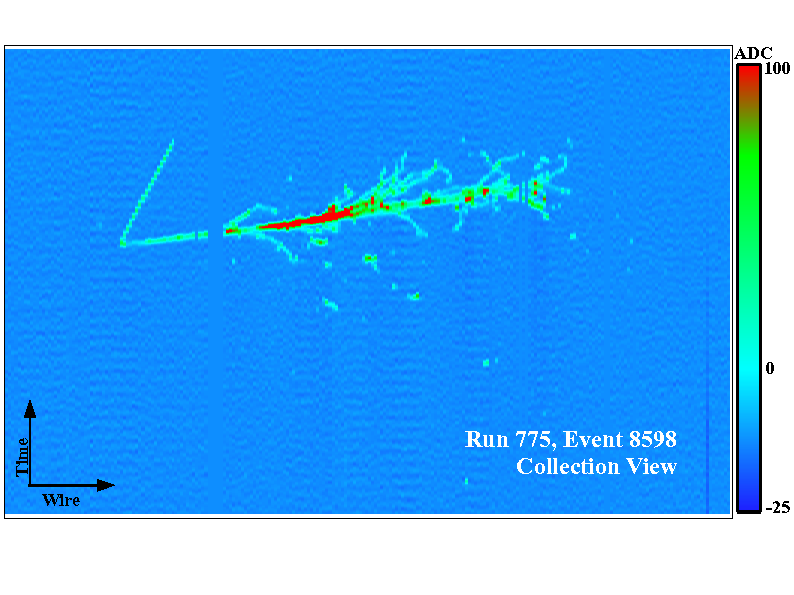
\includegraphics[width=\textwidth]{figs/electron.png}
	\caption{Example of a $\nu_e$ CC event.}
	\label{fig:electron}
	\end{subfigure}
\caption{ArgoNeuT $e/\gamma$ topologies \cite{argoneut5}}
\label{fig:egamma}
\end{figure}

\subsection{Cross sections}
MicroBooNE's neutrino cross-section program will be the first $\nu-Ar$ cross-section in the 1 GeV energy range and one of only a few cross-section measurements of $\nu-Ar$ in the world. MicroBooNE is also the first liquid argon detector to collect the highest statistics sample of neutrino interactions. Investigating final-state-interactions in the 1 GeV energy range provides information about short range nuclear correlations that affect the interpretations of neutrino oscillation experiment data. 

One of the cross-section measurements MicroBooNE can make is an inclusive charged-current cross-section measurement (referred to as CC-inclusive). CC-inclusive events consist of a neutrino exchanging a $W^{\pm}$ boson with an argon atom, producing a charged lepton and any number of other final state particles. In MicroBooNE's case, a CC-inclusive event will mostly have a defining muon track coming out of the vertex due to our neutrinos being predominately $\nu_{\mu}$s. A cross-section measurement is the energy dependent probability of $\nu-Ar$ interaction in the detector. Cross-sections however are independent of the intensity or focus of the particle beam so they can be compared among different experiments. A background for a CC-inclusive cross-section measurement are the neutral-current events that contain a pion. It is possible to have a neutral current interaction with a $\pi+p$ event signature that looks like a charged current $\mu+p$ event. Reconstruction tools implemented to date don't efficiently separate muons from pions. A common way to separate these two particles species is to implement a track length cut. On average, muons tend to have longer track lengths in LArTPCs so by requiring that the hypothesized lepton be above a threshold track length, it is possible to increase signal to background.

\subsection{Liquid argon detector development}
The last physics goal for the MicroBooNE collaboration is to provide important information regarding LArTPC technology. Being the first large scale LArTPCs in the US, MicroBooNE will be able to provide improvements to High Voltage (HV) distribution, Noise Characterization \cite{noisechar}, and Michel Electron Reconstruction \cite{michel}. 

\section{The Booster Neutrino Beam}
The MicroBooNE detector is stationed at Fermilab where it receives neutrinos from both the BNB and NuMI beams. MicroBooNE is on-axis for the BNB and off-axis by 135 mrad for NuMI. For the purpose of this analysis, only data from the BNB was used. This section will discuss how neutrinos are created using the BNB. How these neutrinos are produced as well as their flux through the MicroBooNE detector is necessary for any analysis because of the systematic uncertainties the beam introduces to a cross-section measurement. An aerial view of Fermilab as well as the BNB is shown in figure \ref{fig:fnal}.

\begin{figure}[htp!]
\centering
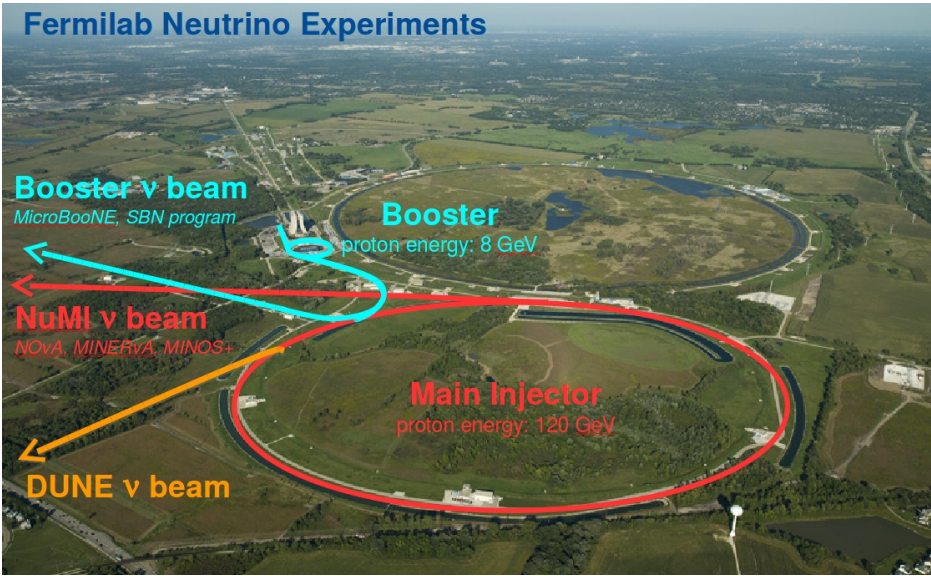
\includegraphics[width=\textwidth]{figs/fnal.png}
\caption{Aerial view of the Main Injector and the Booster Neutrino Beam at Fermilab}
\label{fig:fnal}
\end{figure}

\subsection{Creating the Booster Neutrino Beam}
The BNB is a very pure $\nu_{\mu}$ beam, with only 0.6\% contamination from $\nu_{e}$. The energy also peaks around 700 MeV which is desired based on the probability of oscillation equation which depends on the value of $L/E$, where $L$ is the distance of the detector from the neutrino beam and $E$ is the energy of the neutrino beam. $L/E$ was chosen to match the LSND experiment. The BNB collides 8.9 GeV/c momentum protons from the FNAL booster synchrotron into a beryllium target which produces a high flux of neutrinos. The protons originate from $H^2$ gas molecules that are turned into $H^-$ ions by a Cockroft-Walton generator. The $H^-$ initially are accelerated to 1 MeV kinetic energy and are then passed to a linear accelerator using alternating electromagnetic fields to increase their energy to ~400 MeV. The ions are stripped of electrons by passing them through a carbon foil. The protons are bunched into beam spills which contain ~$4*10^{12}$ protons in a 1.6 $\micro s$ time window per spill. 
It's at this point that the protons are directed towards the beryllium target. The amount of protons directed towards the target (POT) is measured by two toroids upstream of the target with an error of ~2$\%$. Beam intensity, timing, width, position, and direction are monitored by beam position monitors, multi-wire chamber and resistive monitors. 

The beryllium target is 71.1 cm long, 1.7 proton interaction lengths, and is 0.51 cm in radius. The target is located inside a larger focusing electromagnet called the horn. The horn is an aluminum alloy pulsed toroidal electromagnet. The pulsed current peaks at 170 kA with a time-width of 143 $\micro s$ which coincides with the protons arriving on the target. The current flows from the inner conductor to the outer conductor with a maximum magnetic field of 1.5 Tesla. The magnetic field focuses the charged secondary particles produced by the p-Be interactions. The direction of current can be switched to changed to polarity of the secondary particles being focused creating a beam of either primarily neutrinos, with positively charged secondary particles, or anti-neutrinos. 

Further down the beam-line is a concrete collimator which absorbs particles not necessary to the neutrino flux. The collimator is 214 cm long and \sim 30 cm in radius. After the collimator comes a 45 meter long, 1 meter radius, air-filled cylindrical decay region which then ends in a beam-stop made of steam and concrete. The beam-stop contains an array of gas proportional counters to detect muons. The BNB is shown in figure \ref{fig:bnb}.      

\begin{figure}[htp!]
\centering
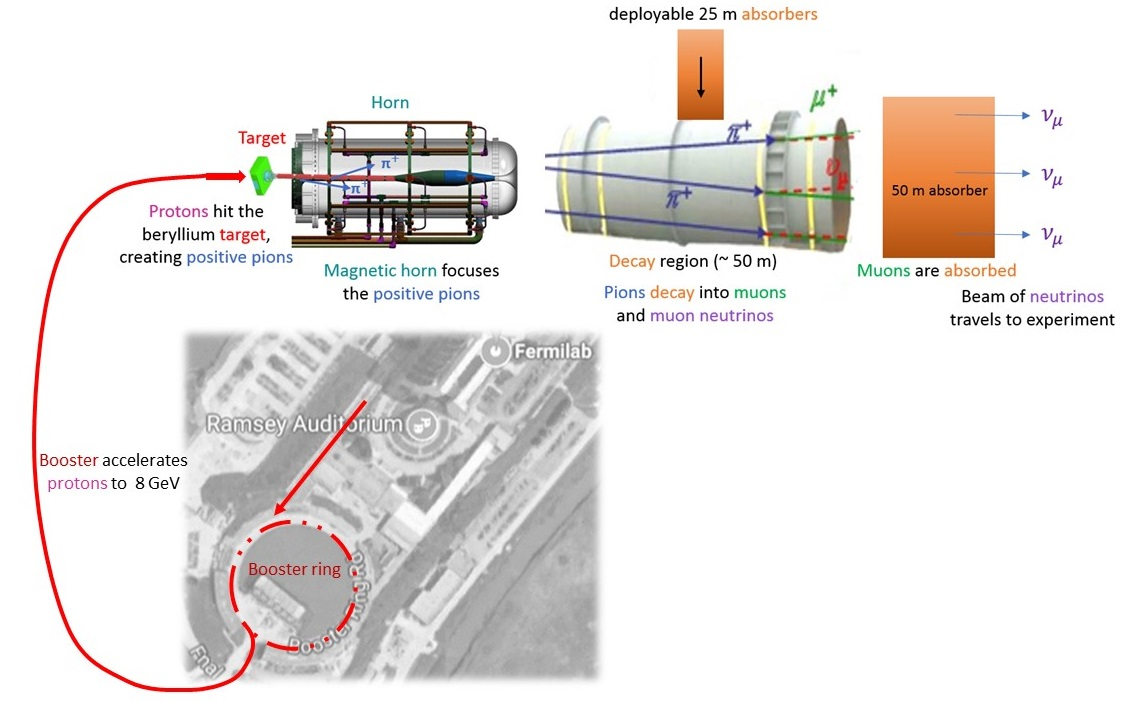
\includegraphics[width=.9\textwidth]{figs/BNB_layout.jpg}
\caption{Depiction of how the Booster Neutrino Beam is made.}
\label{fig:bnb}
\end{figure}

The neutrino flux through MicroBooNE was modeled using Geant4 MC simulation of the beam-line, focusing horn, and decay region. The BNB flux is shown in figure \ref{fig:bnbflux} \cite{neutrinoflux}. 

\begin{figure}[htp!]
\centering
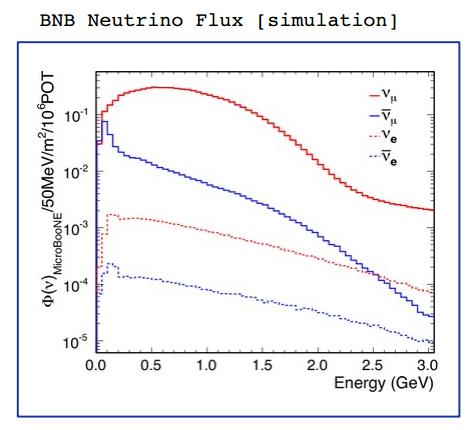
\includegraphics[width=.6\textwidth]{figs/bnbflux.png}
\caption{Energy spectrum of the Booster Neutrino Beam at Fermi National Laboratories \cite{neutrinoflux}}
\label{fig:bnbflux}
\end{figure}


